\chapter{Implementazione}

L'implementazione deve rappresentare una simulazione deterministica. Per questo motivo non sono stati usati tread (oggetti Java \texttt{Thread}).

%%%%%%%%%%%%%%%%%%%%%%%%%%%%%%%%%%%%%%%%%%%%%%%%%%%%%%%%%%%%
\section{Scheduler}
Ogni possibile implementazione di un algoritmo di scheduling è un'estensione della classe \texttt{Scheduler}. Questo permette di definire i comportamenti comuni a tutti gli scheduler e di astrarre future implementazioni.

Per l'implementazione, oltre a ciò che definisce uno scheduler (i.e., taskSet e l'eventuale protocollo di accesso alle risorse), è stato necessario mantenere una lista di task pronti \texttt{readyTaskse} una di task bloccati \texttt{blockedTask}. Inoltre è necessario mantenere un riferimento all'ultimo task che è andato in esecuzione.

\myskip

Nella classe base sono presenti, oltre che ai classici getter e setter, anche i metodi fondamentali che ogni sotto classe deve implementare: \texttt{schedule} che definisce la politica di scheduling; \texttt{assignPriority} che definisce come assegnare la priorità ai task.

Quando uno scheduler viene creato oltre a assegnare il taskset e il protocollo di accesso alle risorse, viene chiamato \texttt{assignPriority}, e vengono inizializzate le strutture relative al protocollo. La scelta di fare questo assegnamento qua e non nella classe dedicata al protocollo è dovuta alle dipendenze: per come è stato implementato l'oggetto principale (e anche l'ultimo che deve essere istanziato) è lo scheduler, e quindi è il protocollo si basa su di esso.

\subsection{Rate Monotonic}
Descriviamo brevemente l'idea di implementazione di RM. Per semplificare l'ordine con cui i vari componenti interagiscono è stato definito il sequence diagram in Figura \ref{fig:sdRM}.

\myskip

Dopo aver chiamato il costruttore della superclasse, RM valuta se tutti i task che compongono il taskset sono puramente periodici, cioè se hanno stesso periodo e deadline relativa.

\begin{figure}[htbp]
    \centering
    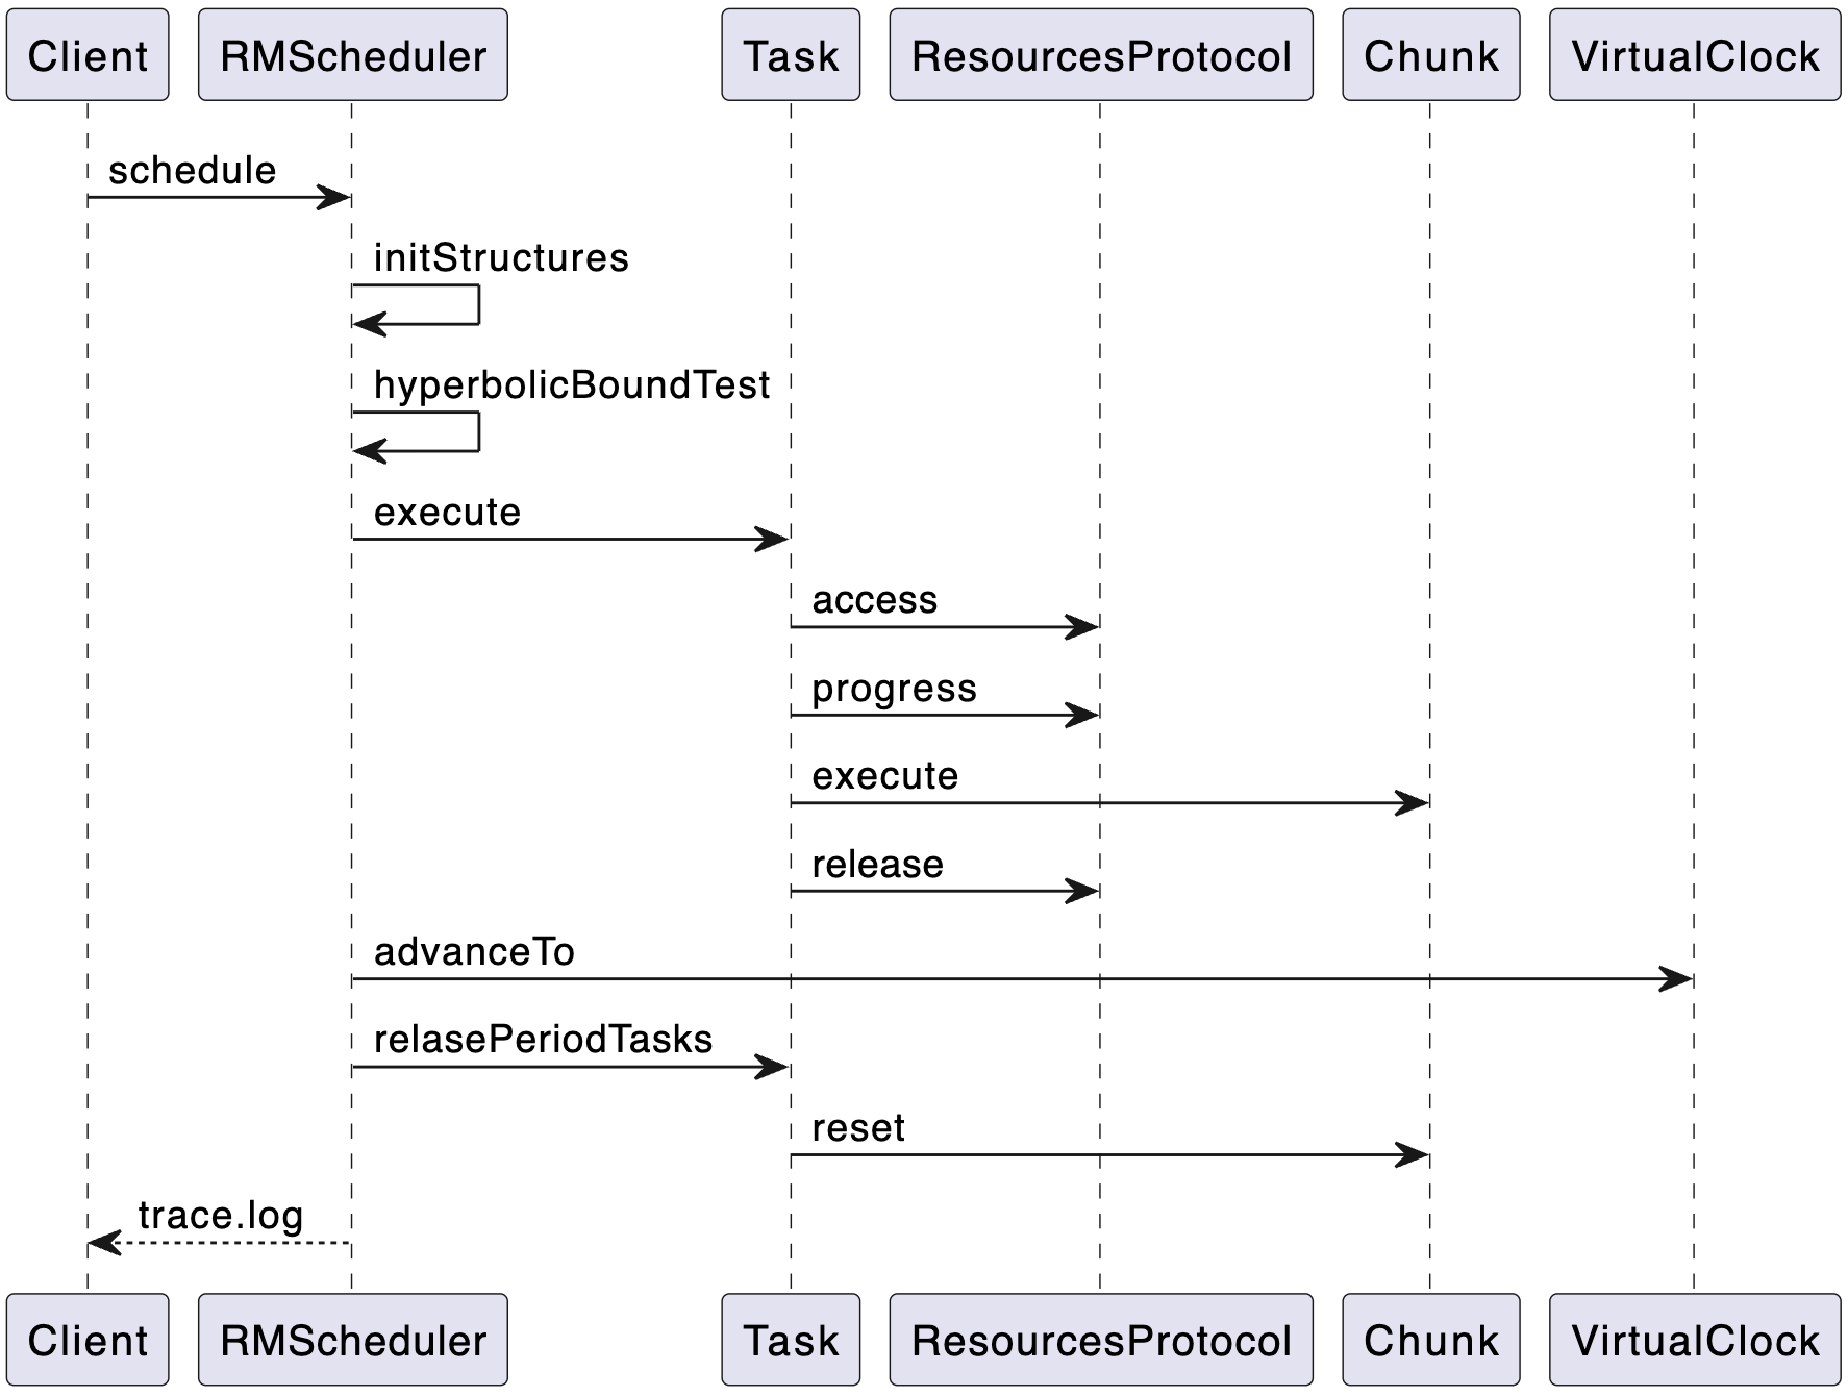
\includegraphics[width=1\textwidth]{immagini/sequence diagram RM.pdf}
    \caption{Sequence Siagram RM}
    \label{fig:sdRM}
\end{figure}

\myskip

La simulazione di scheduling si basa su due strutture principali:
\begin{itemize}
    \item \texttt{taskReady} \\
        Ospita i task che si contendono l'accesso alla CPU. È stata implementa tramite un \texttt{Treeset} e al suo interno si mantiene un'ordinamento inverso rispetto alla durata del periodo dei vari task: task con periodo inferiore ha una priorità maggiore.
    \item \texttt{events} \\
        Gestisce gli eventi rilevanti per lo scheduler, cioè i momenti in cui deve valutare se i task che hanno terminato il periodo hanno superato la deadline oppure se devono essere rilasciati nuovamente. Nell'intervallo tra un perido e il successivo infatti lo scheduler non fa altro che mandare in esecuzione uno dopo l'altro il task a priorità maggiore. Gli eventi sono l’unione ordinata dei multipli di ciascun periodo fino al minimo comune multiplo dei periodi oppure fino a 10 volte il periodo maggiore (per semplicità del caso sia molto oneroso generare questa lista).
\end{itemize}

\myskip

Il metodo \texttt{schedule} poi delega la gestione dei chunk di ogni task alla classe \texttt{Task}, la quale a sua volta rimanda alla calsse \texttt{Chunk} la loro esecuzione (i.e. il logging).

%%%%%%%%%%%%%%%%%%%%%%%%%%%%%%%%%%%%%%%%%%%%%%%%%%%%%%%%%%%%
\section{Resource Access Protocol}
Ogni implementazione di un protocollo di accesso alle risorse deve estendere la classe \texttt{ResourceProtocol}.

l'idea iniziale era di implementare il concetto astratto di protocollo di accesso tramite un'interfaccia, ma vista la necessità di mantenere un riferimento allora scheduler nel protocollo si è introddo questo campo nella classe base.

\myskip

I metodi definiti da questa classe astratta sono le operazioni che devono essere svolte da un procotollo di questo tipo: deve gestire la fase di accesso, progresso e rilascio. Definisce anche il metodo \texttt{initStructures} che ha il compito di inizializzare le strutture dati usate dal protocollo.

Oltre a questi metodi è dichiarato un metodo \texttt{initStructures} che inizializza le strutture necessarie al protocollo.

\subsection{Priority Ceiling Protocol}
Tralasciando quello che fanno i metodi di accesso, progresso e rilascio, che riflettono quanto ci dice la teoria, in questo classe le strutture usate sono prevalentemente due:
\begin{itemize}
    \item \texttt{ceiling} \\
        È una mappa che associata ad ogni risorsa il suo ceiling, cioè la massima priorità nominale dei task che usano quella risorsa.
    \item \texttt{busyResources}\\
        È una lista delle risorse che sono occupate da un qualche task.
\end{itemize}

%%%%%%%%%%%%%%%%%%%%%%%%%%%%%%%%%%%%%%%%%%%%%%%%%%%%%%%%%%%%
\section{Utilità}
Vediamo la scelta su alcuni componenti di utilità.

\subsection{Loggin}
Per il logging è stato implementato un semplice logging su un file e viene rappresnetato come una sequenza di coppie $<evento,tempo>$.

Il file di destinazione delle tracce loggate è \texttt{trace.log}.

\subsection{Clock}
Il tempo all'interno del sistema è gestito globalmente: ad ogni esecuzione del \texttt{main} il tempo viene resettato. Questa scelta è dovuta al fatto che praticamente tutti gli ogegtti devono accedere al clock del sistema; in questo modo si evita di passarlo ogni volta nei vari metodi chiamati a cascata. L'implementazione è stata fatta tramite il pattern Singleton.

A causa della staticità si consiglia di usare eseguire una sola simulazione per esecuzione. C'è la possibilità di resettarlo manualmente (tramite \texttt{MyClock.reset()}); questa possibilità è stata introdotto per i test.

Il clock del sistema è rappresnetato dalla classe \texttt{MyClock}. Questa non fa altro che mantenere il tempo assoluto ed esporre due metodi che permettono di avanzare di un dato intervallo temporale e avanzare fino a un determinato tempo.

\myskip

Il tempo è gestito tramite oggetti di tipo \texttt{Duration}, classe di \texttt{java.time} che implementa oggetti immutabili e che permetto una facile gestione del tempo.

\subsection{Sampling dei tempi}
Quando si deve definire i tempi che definiscono i vari componenti del sistema, cioè come il periodo, la dealine, l'execution time di un chunk, si usa un campionamento da un data distribuzione.

Le distribuzioni sono implementate dalla libreria \texttt{Sirio}; oltre a quelle definite dalla libreria è stata implementata la classe \texttt{ConstantSampler}, che permette di gestire tempi costanti, mantenendo l'astrazione della libreria Sirio.

\subsection{Eccezioni}
Durante l'esecuzione si possono verificare dei problemi, più o meno previsti. Questi sono gestiti tramite eccezioni; questo permette in futuro di cambiare o aggiungere un comportamente del sistema quando si verificano determinate situazioni.

\myskip

Le eccezioni implementate è utili sono:
\begin{itemize}
    \item \texttt{DeadlineMissedExeption} \\
        Viene sollevata quando un task non rispetta la deadline. Il sistema non la gestisce, ma la propaga fino al main: in questo modo se e quando si verifica questo problema, viene stamapta in \texttt{trace.log} e la simulazione si arresta.
    \item \texttt{AccessResourceProtocolExeption} \\
        Viene sollevata quando un task viene bloccato dal metodo \texttt{access} del protocollo di accesso.
\end{itemize}